%------------------ vorlage.tex ------------------------------------------------
%
% LaTeX-Vorlage zur Erstellung von Projektdokumentationen
% im Fachbereich Informatik der Hochschule Trier
%
% Basis: Vorlage 'svmono' des Springer Verlags
% Bearbeiter: Hermann Schloß, Christian Bettinger
%
%-------------------------------------------------------------------------------


%------------------ Präambel ---------------------------------------------------
\documentclass[envcountsame, envcountchap, deutsch]{i-studis}

\usepackage[utf8]{inputenc}

\usepackage[a4paper]{geometry}
\usepackage[english, ngerman]{babel}

\usepackage[pdftex]{graphicx}
\usepackage{epstopdf}

\usepackage{listings}

\usepackage[german, ruled, vlined]{algorithm2e}
\usepackage{amssymb, amsfonts, amstext, amsmath}
\usepackage{array}
\usepackage[skip=10pt]{caption}
\usepackage[usenames, dvipsnames]{color}
\usepackage[pdftex, plainpages=false]{hyperref}
\usepackage{textcomp}

\usepackage{bibgerm}
\bibliographystyle{geralpha}

\usepackage{makeidx}
\usepackage{multicol}
\makeindex

\pagestyle{myheadings}
\setlength{\textheight}{1.1\textheight}

\lstset{
	basicstyle=\scriptsize\ttfamily,
	commentstyle=\scriptsize\ttfamily\color{Gray},
	identifierstyle=\scriptsize\ttfamily,
	keywordstyle=\scriptsize\ttfamily,
	stringstyle=\scriptsize\ttfamily,
	tabsize=4,
	numbers=left,
	numberstyle=\tiny,
	numberblanklines=false,
	frame=single,
	framesep=3mm,
	framexleftmargin=7mm,
	xleftmargin=10mm,
	linewidth=144mm,
	captionpos=b,
}


%------------------ Manuelle Silbentrennung ------------------------------------
\hyphenation{Ele-men-tar-ob-jek-te ab-ge-tas-tet Aus-wer-tung House-holder-Matrix Least-Squares-Al-go-ri-th-men}


%------------------ Titelseite -------------------------------------------------
\begin{document}

\title{Entwicklung einer Hotelbuchungssoftware}
\subtitle{Development of hotel booking software}

\author{Alexander Falkenberg, Hasan Alhelal}

\supervisor{Titel Vorname Nachname}

\address{Ort}
\submitdate{DD.MM.YYYY}

%------------------ Projektart -------------------------------------------------
%\project{Bachelor-Projektarbeit}
\project{Teamprojekt}
%\project{Master-Projektstudium}
%\project{Master-Abschlussarbeit}
%\project{Seminar}
%\project{Hausarbeit}

\mytitlepage

%------------------ Vorwort, Kurzfassung, Verzeichnisse ------------------------
\frontmatter					% Vorwort (optional)
\kurzfassung

In der Kurzfassung soll in kurzer und prägnanter Weise der wesentliche Inhalt der Arbeit beschrieben werden. Dazu zählen vor allem eine kurze Aufgabenbeschreibung, der Lösungsansatz sowie die wesentlichen Ergebnisse der Arbeit. Ein häufiger Fehler für die Kurzfassung ist, dass lediglich die Aufgabenbeschreibung (d.h. das Problem) in Kurzform vorgelegt wird. Die Kurzfassung soll aber die gesamte Arbeit widerspiegeln. Deshalb sind vor allem die erzielten Ergebnisse darzustellen. Die Kurzfassung soll etwa eine halbe bis ganze DIN-A4-Seite umfassen.

Hinweis: Schreiben Sie die Kurzfassung am Ende der Arbeit, denn eventuell ist Ihnen beim Schreiben erst vollends klar geworden, was das Wesentliche der Arbeit ist bzw. welche Schwerpunkte Sie bei der Arbeit gesetzt haben. Andernfalls laufen Sie Gefahr, dass die Kurzfassung nicht zum Rest der Arbeit passt.

\kurzfassungEN

The same in English.
							% Kurzfassung/Abstract
\tableofcontents										% Inhaltsverzeichnis
\listoffigures											% Abbildungsverzeichnis (optional)


%------------------ Kapitel ----------------------------------------------------
\mainmatter
\chapter{Einleitung}
\section{Motivation}
Diese Arbeit handelt von der Umsetzung eines Buchungssystems für ein Hotel. Ein solches System ist besonders wichtig um den allgemeinen Aufwand beim Verwalten von verfügbaren Zimmern deutlich zu verringern und der Fehleranfälligkeit beim Vergeben von eben diesen vorzubeugen. Unternehmen profitieren von solchen Software-Lösungen, da Mitarbeiter entlastet werden und Kunden leichter eine Buchung tätigen können. Außerdem kann diese Software in leicht abgeänderter Form auch problemlos für andere Anwendungen oder Unternehmen mit anderen Produkten oder Dienstleistungen benutzt werden.


\section{Ziele der Arbeit}
Ziel dieser Arbeit ist es ein simples Buchungssystem zu schaffen dass sich ohne großen Arbeitsaufwand verwenden lässt. Es soll den Nutzern des Systems möglich sein, ohne die Erstellung eines Nutzerprofils Buchungen tätigen und diese verwalten zu können. Die Informationen über jede Buchung werden den Nutzern anschließend per Email zugesandt. Ein Nutzer soll außerdem die Möglichkeit haben, alle Infos sowie 3D-Modelle der Zimmer abrufen und Bewerbungen über die Anwendung zu versenden.
\chapter{Verwandte Arbeiten}

Die Gliederung hängt natürlich vom Thema und von der Lösungsstrategie ab. Als nützliche Anhaltspunkte können die Entwicklungsstufen oder -schritte z.B. der Software-Entwicklung betrachtet werden. Nützliche Gesichtspunkte erhält und erkennt man, wenn man sich

\begin{itemize}
	\item in die Rolle des Lesers oder
	\item in die Rolle des Entwicklers, der die Arbeit z.B. fortsetzen, ergänzen oder pflegen soll,
\end{itemize}

versetzt. In der Regel wird vorausgesetzt, dass die Leser einen fachlichen Hintergrund haben - z.B. Informatik studiert haben. D.h. nur in besonderen, abgesprochenen Fällen schreibt man in populärer Sprache, so dass auch Nicht-Fachleute die Ausarbeitung prinzipiell lesen und verstehen können.

Die äußere Gestaltung der Ausarbeitung hinsichtlich Abschnittformate, Abbildungen, mathematische Formeln usw. wird in Kapitel \ref{Bausteine} kurz dargestellt.

\chapter{Grundlagen}

\section{HTML, CSS, JS}
\subsection{HTML}
\subsection{Less}
\subsection{JavaScript}

\section{Node.js}
Die serverseitige Grundlage des Systems bildet die Laufzeitumgebung Node.js. Mit dieser ist es möglich JavaScript Programme abseits eines Browsers ausführen zu können. Mithilfe von \glqq npm\grqq, dem Paketmanager von Node.js, werden außerdem externe Pakete für bestimmte Funktionalitäten verwendet um die Implementierung zu vereinfachen.

\subsection{Express}
Das Express-Framework ermöglicht eine unkomplizierte Erstellung einer Webanwendung. So wird beispielsweise die Verarbeitung von HTTP-Anfragen wird mithilfe von spezifischen Methoden deutlich vereinfacht und macht das Erstellen einer API besonders effizient. Innerhalb der Buchungssoftware sorgt Express für die Bereitstellung eines Servers, der alle clientseitigen Dateien zur Verfügung stellt und auf HTTP-Anfragen zur Erzeugung oder zum Abrufen von Buchungen, reagiert.

\subsection{Nodemailer}
Nodemailer ist ein \glqq npm\grqq-Paket, das dafür verwendet wird E-Mails mit Node.js zu versenden. Durch Angabe der Adresse von der die E-Mail verschickt werden soll und verschiedenen Optionen wie z.B. dem Betreff wird das Senden vereinfacht. Um eine E-Mail zu versenden muss im ersten Schritt ein \glqq Transporter\grqq zusammen mit dem verwendeten Mail Dienst und den Anmeldeinformationen der zu sendenen E-Mail Adresse, erzeugt werden. Anschließend werden die Mail-Optionen initialisiert und über die Methode \glqq sendMail\grqq des Transportes, die E-Mail versandt.

\subsection{Formidable}

\section{MongoDB}
Unter den dokumentenorientierten NoSQL-Datenbanken ist MongoDB die meist verwendete. Die wichtigsten Bestandteile einer MongoDB Datenbank sind Dokumente und Collections. Dokumente sind Datenstrukturen die sich aus einem oder mehreren Paaren, bestehend aus Feldern und dazugehörigen Werten, zusammenfügen. In ihrem Aufbau sind diese Dokumente identisch mit JSON Objekten. Collections hingegen sind Sammlungen von verschiedenen Dokumenten und sind vergleichbar mit Tabellen aus relationalen Datenbanken.
\\
\\
Damit eine Node.js-Anwendung mit einer MongoDB kommunizieren kann wird beispielsweise das \glqq npm\grqq-Paket \glqq mongodb\grqq benötigt. Hier können dann auf den einzelnen Collections, Methoden angwendet werden. Die wichtigsten Methoden für das zu erstellende System sind \glqq find\grqq , \glqq insertOne\grqq , \glqq deleteOne\grqq und \glqq deleteMany\grqq. Mithilfe von find werden alle Dokumente einer Collection geliefert, auf die ein in der Methode spezifiziertes Kriterium zutrifft. InsertOne ermöglicht es ein neues Dokument in eine Collection hinzuzufügen und deleteOne bzw. deleteMany ermöglicht das Löschen von Dokumenten aus einer Collection.

\chapter{Konzept}

\begin{figure}
	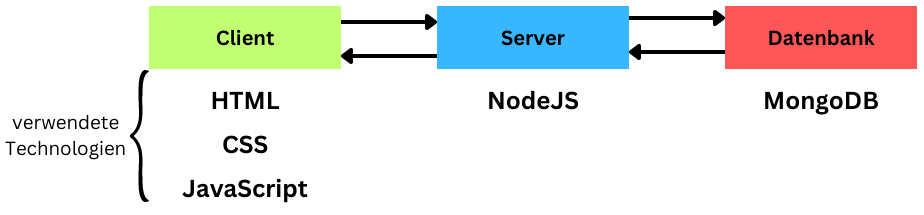
\includegraphics[width=\textwidth]{images/Architektur.png}
	\caption{Grobe Architektur des Systems}
\end{figure}

\chapter{Realisierung}
\section{Buchung}



\chapter{Implementierung}
\section{Buchungsdialog}
Dem Client soll es innerhalb der Anwendung ermöglicht werden über einen \glqq Buchungsdialog\grqq \thickspace eine Buchung abzuwickeln. Dieser Dialog teilt sich in mehrere Schritte auf. Im ersten Schritt muss der Nutzer ein Formular, bestehend aus Ankunfts-, Abreisedatum, Anzahl der Erwachsenen, Anzahl der Kinder und die Anzahl der Räume, ausfüllen. Will der Nutzer nun mit dem zweiten Schritt fortführen werden zuerst die Eingaben aus dem ersten Schritt auf Gültigkeit geprüft. Gültigkeit heißt in diesem Fall dass beispielsweise das Ankunftsdatum nicht in der Vergangenheit oder vor dem Abreisedatum liegen darf. Sind die Eingaben gültig wird eine HTTP-Anfrage an den Server geschickt mit dem Ziel alle zu der angegeben Aufenthaltszeit verfügbaren Zimmer als HTTP-Antwort zu erhalten. Im zweiten Schritt des Dialogs kann der Nutzer aus allen verfügbaren Zimmern die passenden für seinen Aufenthalt wählen. Bevor mit dem dritten Schritt fortgeführt wird, muss geprüft werden das genau so viele Zimmer, wie im ersten Schritt angegeben, ausgewählt wurden. Ist dies der Fall wird im nächsten Schritt mit einem Formular für alle persönlichen Daten des Nutzers fortgesetzt. Werden alle Felder des Formulars ordnungsgemäß ausgefüllt kann mit dem vierten und letzten Schritt fortgeführt werden. In diesem wird dem Nutzer eine Übersicht der angegebenen Daten bzw. der Buchung angezeigt und bietet dem Nutzer über ein Textfeld die Möglichkeit Extrawünsche an das Hotel zu äußern. Will der Nutzer die Buchung abschließen wird eine HTTP-POST-Anfrage an den Server, mit allen wichtigen Daten zu Erstellung der Buchung, versendet.

\section{Meine Buchung}
In der Webanwendung wird einem Nutzer unter dem Punkt \glqq Meine Buchung\grqq \thickspace ermöglicht Informationen über getätigte Buchungen abzufragen und diese Anzupassen. Hierfür muss in ein dafür bestimmtes Feld die Buchungsnummer des Clients eingegeben werden. Anschließend wird eine HTTP-GET-Anfrage mit dem Pfad \glqq /order/:id\grqq \thickspace an den Server gesendet, auf die der Server mit allen Informationen zu der Buchung antwortet, wenn die Buchungsnummer existiert. Im Anschluss wird dem Nutzer eine Übersicht mit den wichtigsten Informationen dargeboten und zusätzlich die Möglichkeit die Buchung zu stornieren oder die Reisedaten abzuändern.
\\
\\
Entscheidet sich der Client dazu die Buchung zu stornieren wird einem Fenster-Alert gefragt ob sich der Nutzer mit der Stornierung sicher ist. Bestätigt der Client die Löschung wird eine HTTP-DELETE-Anfrage mit dem Pfad \glqq /order/:id\grqq \thickspace an den Server gesendet. Ist die Stornierung erfolgreich wird eine Bestätigungs-E-Mail an den Nutzer gesendet.
\\
\\
Wird sich jedoch für die Änderung der Daten entschieden wird in einem neuen Fenster ein Formular zur Eingabe der neuen Reisedaten angezeigt. Werden dort die neuen Daten eingegeben und fortgefahren, sendet der Client eine HTTP-POST-Anfrage mit dem Pfad \glqq /order/dates\grqq \thickspace an den Server versendet.

\section{Buchung API}
Serverseitig wird eine API erstellt, die die clientseitige Kommunikation mit dem Server ermöglicht. Dafür wird ein express-Router mit verschiedenen Routen benötigt, die unter anderem das Erstellen, Löschen, Verändern und Abfragen von Buchungen abwickeln. Ein solcher Router wird mit express-Methode \glqq express.Router()\grqq \thinspace erstellt. Für jede Route wird es außerdem von Nöten sein, Zugriff auf die MongoDB-Datenbank zu besitzen. Mithilfe des MongoDB-Moduls wird dafür ein \glqq MongoClient\grqq \thinspace erzeugt, der die Adresse der MongoDB-Datenbank übergeben bekommt.

\subsection{Erstellen einer Buchung}
Für die Erstellung einer Buchung wird dem Router eine Route hinzugefügt, die auf einen HTTP-POST mit dem Pfad \glqq /order \grqq \thinspace reagiert. Innerhalb der Funktion die die Anfrage behandelt werden zu aller erst alle für die Buchung benötigten Informationen aus dem Request-Objekt in Konstanten gespeichert. Zu den benötigten Informationen gehören: Vorname, Nachname, E-Mail-Adresse, Telefonnummer, Wohnort (mit Ort, Straße, Hausnummer und PLZ), Ankunftsdatum, Abreisedatum und die Art von Zimmern die gebucht werden sollen. Anschließend wird geprüft ob die Konstanten gültig sind. Sollte eine nicht zulässig sein wird eine HTTP-Antwort mit dem Code 400 an den Client gesendet. Bestehen jedoch alle Konstanten die Prüfung, wird mit der Verbindung des MongoClients fortgeführt. Der Aufruf der \glqq connect\grqq- und daraufhin der \glqq db\grqq-Methode (mit dem Namen der gesuchten Datenbank) des bereits erstellten MongoClients, liefert ein Datenbank-Objekt mit dem nun einzelne Collections abgerufen werden können. 
\\
\\
Um einen neuen Nutzer anzulegen muss ein Collection-Objekt zur Anpassung der Collection die alle Nutzer enthält, mithilfe der \glqq collection\grqq -Methode des Datenbank-Objekts, erzeugt werden. Das Collection-Objekt erlaubt es mit der Methode \glqq insertOne(elemToInsert)\grqq \thinspace den neuen Nutzer mit allen dazugehörigen Informationen aus den gespeicherten Konstanten (Vorname, Nachname, Adresse, E-Mail, Telefonnummer) in die Collection einzufügen.
\\
\\
Im weiteren Verlauf werden die Collection mit allen Buchungen und die Collection mit allen Zimmern benötigt. Werden auf beiden Collections jeweils die Methoden \glqq find().toArray()\grqq \thinspace ohne Parameter aufgerufen, können alle Buchungen und Zimmer als Feld in jeweiligen Variablen abgelegt werden. Mithilfe des Algorithmus in \ref{alg:one} werden alle zu der angegebenen Ankunfts- und Abreisezeit verfügbaren Zimmer geliefert. Sind genug Zimmer mit den vom Client angegebenen Zimmertypen nicht vergeben werden für jeden zu buchenden Raum eine neue Buchung in die Buchungs-Collection eingefügt. Dabei besteht jede Buchung aus der ID des neuen Nutzers, der ID des verfügbaren Raums, des Ankunfts- und Abreisedatums.
\\
\\
Zuletzt wird per nodemailer eine Mail an die E-Mail-Adresse des Clients gesendet. Diese enthält die ID des angelegten Nutzers, welche später zu Änderung oder Stornierung der Buchung verwendet werden kann. Als Antwort erhält der Client eine HTTP-Antwort mit dem Status-Code 200 insofern keine Komplikationen auftreten.

\subsection{Ändern einer Buchung}
Um einem Nutzer zu ermöglichen die Daten einer bereits getätigten Buchung zu ändern, wird eine Route hinzugefügt, die auf einen HTTP-POST mit dem Pfad \glqq /order/dates\grqq \thinspace reagiert. Dafür müssen im ersten Schritt die Variablen mit den Werten aus dem HTTP-Body initialisiert und anschließend auf Gültigkeit überprüft werden. Die Werte bestehen aus der ID des Nutzers, das neue Ankunfts- und Abreisedatum. Sollte einer der Werte ungültig sein, wird eine HTTP-Antwort mit dem Status-Code 400 an den Client versendet. Sind sie jedoch gültig verbindet sich der MongoClient mit der Datenbank und fordert alle Buchungen an. Anschließend werden mithilfe der find-Methode einerseits alle Buchungen die mit der ID des Nutzers übereinstimmen und andererseits alle anderen Buchungen, in zwei verschiedenen Konstanten gespeichert. Aus den Raum-IDs der Buchungen des Nutzers werden alle Räume aus der Raum-Collection die diese IDs besitzen, in einem Feld gesammelt. Dadurch ist es möglich die in der Buchung gebuchten Zimmertypen in Variablen zu speichern, damit bei der Änderung der Daten auch wieder dieselben Zimmertypen gewählt werden. Wie schon in Kapitel 6.1.1 erklärt müssen auch hier alle Zimmer die während des neuen Ankunftsdatum bis zum neuen Abreisedatum verfügbar sind, ermittelt werden.
\\
\\
Sollte es nicht genügend Zimmer mit denselben Zimmertypen wie in der ursprünglichen Buchung geben, die während der neuen Daten verfügbar sind wird die bestehende Buchung nicht geändert und eine HTTP-Antwort mit dem Status-Code 400 an den Client gesendet. Sollte es jedoch genügend Zimmer geben wird die bisherigen Buchungen aus der \glqq reservation\grqq-Collection mithilfe der \glqq deleteMany\grqq-Methode gelöscht und anschließend neue Buchungen der gleichen Zimmertypen zu anderen Zeiten in diese Collection eingefügt. Ist der Ablauf problemlos wird der Status-Code 200 an den Client gesendet.

\subsection{Abfragen einer Buchung}
Um einem Nutzer zu ermöglichen die wichtigsten Daten wie beispielsweise das Ankunftsdatum, Abreisedatum, Anzahl der Nächte, der Gesamtpreis und die Anzahl der Räume einer bereits getätigten Buchung abzurufen, wird eine Route hinzugefügt, die auf einen HTTP-GET mit dem Pfad \glqq /order/:id\grqq \thinspace reagiert. Im ersten Schritt wird die ID der gesuchten Buchung aus den Parametern der HTTP-Anfrage in einer Konstante gespeichert und geprüft ob diese eine gültige MongoDB-ObjectId ist. Wenn die ID zulässig ist werden alle Reservierungen dessen Nutzer-ID mit dieser übereinstimmt in der MongoDB abgerufen. Mithilfe der Buchungen lassen sich das Ankunfts-, Abreisedatum und folglich auch die Anzahl der Nächte ermitteln. Außerdem werden wie schon in 6.1.1 und 6.1.2 alle Räume in Form eines Feldes benötigt. Der Gesamtpreis der Buchung wird dann wie folgt berechnet:
\begin{lstlisting}{Gesamtpreis}
	for (const room of rooms) {
		for (const reservation of reservations) {
			if (room._id.equals(reservation.room)) {
				totalPrice += room.price;
			}
		}
	}
    totalPrice *= totalNights;
\end{lstlisting}
Sind alle Daten zusammengetragen werden diese als JSON mit dem Status-Code 200 an den Client versendet.

\subsection{Löschen einer Buchung}
Für das Löschen einer Buchung wird eine Route benötigt, die auf ein HTTP-DELETE mit dem Pfad \glqq /order/:id\grqq \thickspace reagiert. Zuerst wird die ID der zu löschenden Buchung aus den Parametern der Anfrage auf Gültigkeit geprüft. Anschließend wird der Nutzer der diese ID besitzt, mithilfe der \glqq deleteOne\grqq-Methode der Nutzer-Collection aus dieser entfernt. Außerdem müssen alle Buchungen die diese ID besitzen durch die \glqq deleteMany\grqq-Methode aus der Buchungscollection entfernt werden. Treten keine Probleme bei der Löschung auf wird eine HTTP-Antwort mit dem Status-Code 200 an den Client gesendet.

\section{Bewerbungsformular}
Unter dem Punkt Karriere ist es innerhalb der Anwendung möglich über ein eigens dafür erstelltes Formular eine Bewerbung an den Betreiber der Webanwendung zu senden. Hier soll es unter anderem ermöglicht werden, den Lebenslauf und die Bewerbung als PDF hochzuladen. Beim Absenden des Formulars wird die HTTP-Methode POST mit dem Pfad \glqq \thickspace verwendet. Serverseitig wird eine passende express-Route definiert, in welcher mithilfe von Formidable der Dateien-Upload gewährleistet wird.
\\
\\
Im ersten Schritt wird in der express-Route das eingehende Formular durch \newline \glqq const form = new formidable.IncomingForm()\grqq \thickspace in einer Konstante gespeichert. Anschließend können die Attribute des Formulars zugewiesen werden. In diesem Fall wird festgelegt das mehrere Dateien akzeptiert werden, das jede Datei maximal 5MB groß sein darf und in welchem Ordner die Dateien abgelegt werden. Danach wird folgende Methode aufgerufen: \glqq form.parse(request, CALLBACK)\grqq \thickspace, wobei CALLBACK eine Funktion mit allen Feldern und Dateien des Formulars als Parameter ist. In dieser Funktion wird unter anderem definiert wie mit einem Error umgegangen werden soll. Sollte kein Error auftreten wird mit dem speichern der hochgeladenen Dateien fortgefahren. Dafür wird im ersten Schritt der Dateien-Parameter in eine JSON umgewandelt und alle Schlüssel dieser in einem Feld gespeichert. In einer for-Schleife wird dann durch alle Schlüssel iteriert und unter anderem geprüft ob jede Datei größer als 0MB ist ein gültiges Format besitzt. Sollte die Größe einer der Dateien, 0MB entsprechen wird diese aus dem Dateisystem entfernt und Dateien im falschen Formate sorgen dafür das der Server dem Client mit dem Status-Code 400 antwortet. Ist die Datei gültig wird sie umbenannt und der neue Pfad in einem neuen Feld gespeichert. Anschließend werden die Dateien aus dem neuen Feld per nodemailer an eine E-Mail angehängt und dem Betreiber der Webanwendung gesendet.

\section{Dreidimensionale Zimmer}
Zunächst wird ein Canvas-Element in der HTML Datei benötigt. Diese Element bleibt leer und dient nur als Zeichenfläche für die mit JavaScript bzw. Three.js erstellten Objekte. Als nächstes wird ein Renderer verwedet, der das Ergebnis am Ende in dem Canvas-Element rendert, dazu wird ein Instanz des Renderes wie folgt erzeugt: renderer = new THREE.WebGLRenderer(). Des Weiteren werden zwei weitere Objekte erzeugt, das Szeneobjekt let scene = new THREE.Scene() und das Kameraobjekt let camera = new THREE.PrespectiveCamera(). Diese werden miteinander verbunden in dem sie als Argumente an die Methode renderer.render(scene, camera) übergeben wird. Allerdings müsste diese Methode nach jedem gerenderten Frame aufgerufen werden. Damit es automatisch geschieht eignet sich eine gesonderte namens animate(), in der die vorher erwähnte Funktion einmal aufgerufen wird an den renderer wie folgt zu übergeben: renderer.setAnimationLoop(animate).
\newpage
Das Kameraobjekt hat folgende Parameter:
\begin{enumerate}
	\item \textbf{Field Of View (engl. Sichtfeld)}, hier liegt ein passender Wert zwischen 40-80 Grad.
	\item \textbf{Aspect ratio (engl. Seitenverhältnis)}, mit window.innerWidth / window.innerHeight wird die gerenderte Szene in Vollbild Modus angezeigt und somit die komplette Fläche des Bildschirmes genutzt.  
	\item \textbf{Near (engl. Nahe)}, hier eignet sich ein geringer Wert zwichen 0.1-1, denn jeder Wert darunter wird abgeschnitten. Dieser Parameter besitzt keine Einheit. 
	\item \textbf{Far (engl. Weit)}, hier eignet sich ein hoher Wert wie 1000, denn jeder höhere Wert wird abgeschnitten. Dieser Parameter besitzt keine Einheit.
\end{enumerate}
Das Kameraobjekt befindet standardmäßig an der Position x = 0, y = 0, z = 0. Diese lässt sich aber beliebig mit der Methode \glqq camera.position.set()\grqq \thickspace ändern. Die Instanz der OrbitControls: orbit = new OrbitControls(camera, renderer.domElement), ermögicht den Nutzern die Kamera beliebig zu drehen. Das Orbitobjekt nimmt ein Kameraobjekt und renderer.domElement als Parameter. Damit die Position der Kamera nach einer Mausbewegung aktualisiert wird, wird die Methode orbit.update() aufgerufen.
\\
\\
Die im Projekt verwendeten .hdr-Bilder bieten realistische Beleuchtung, Schatten und Spiegelung. Von daher war es nötig eine Instanz des RGBELoaders: loader = new RGBELoader(), zu erzeugen. Die Methode loader.load nimmt zwei Parameter, der relative Pfad des .hdr-Bilds und eine Rückruffunktion, die eine Textur als Argument hat. Die Textur bzw. das Bild wird dann als Hintergrund der Szene festgelegt.

\chapter{Beispiele}
Im Folgenden wird eine beispielhafte Interaktion eines Nutzers mit dem System anhand von Bildschirmabzügen erläutert. In diesem Szenario will der fiktive Nutzer eine Buchung für Zimmer in dem Grandline-Hotel tätigen. Im ersten Schritt besucht der Nutzer die Startseite und klickt auf den \glqq buchen\grqq-Knopf (siehe Abb.\ref{step1}).
\begin{figure}
	\includegraphics[width=\textwidth]{images/Beispiel/Schritt1.png}
	\caption{Schritt 1}
	\label{step1}
\end{figure}
\newline
Als Folge des Klicks auf den \glqq buchen\grqq-Knopf kommt ein Formular (siehe Abb.\ref{step2}) hervor in welchem der Nutzer die Reisedaten und Anzahl der Zimmer für die gewünschte Buchung angeben kann.
\begin{figure}
	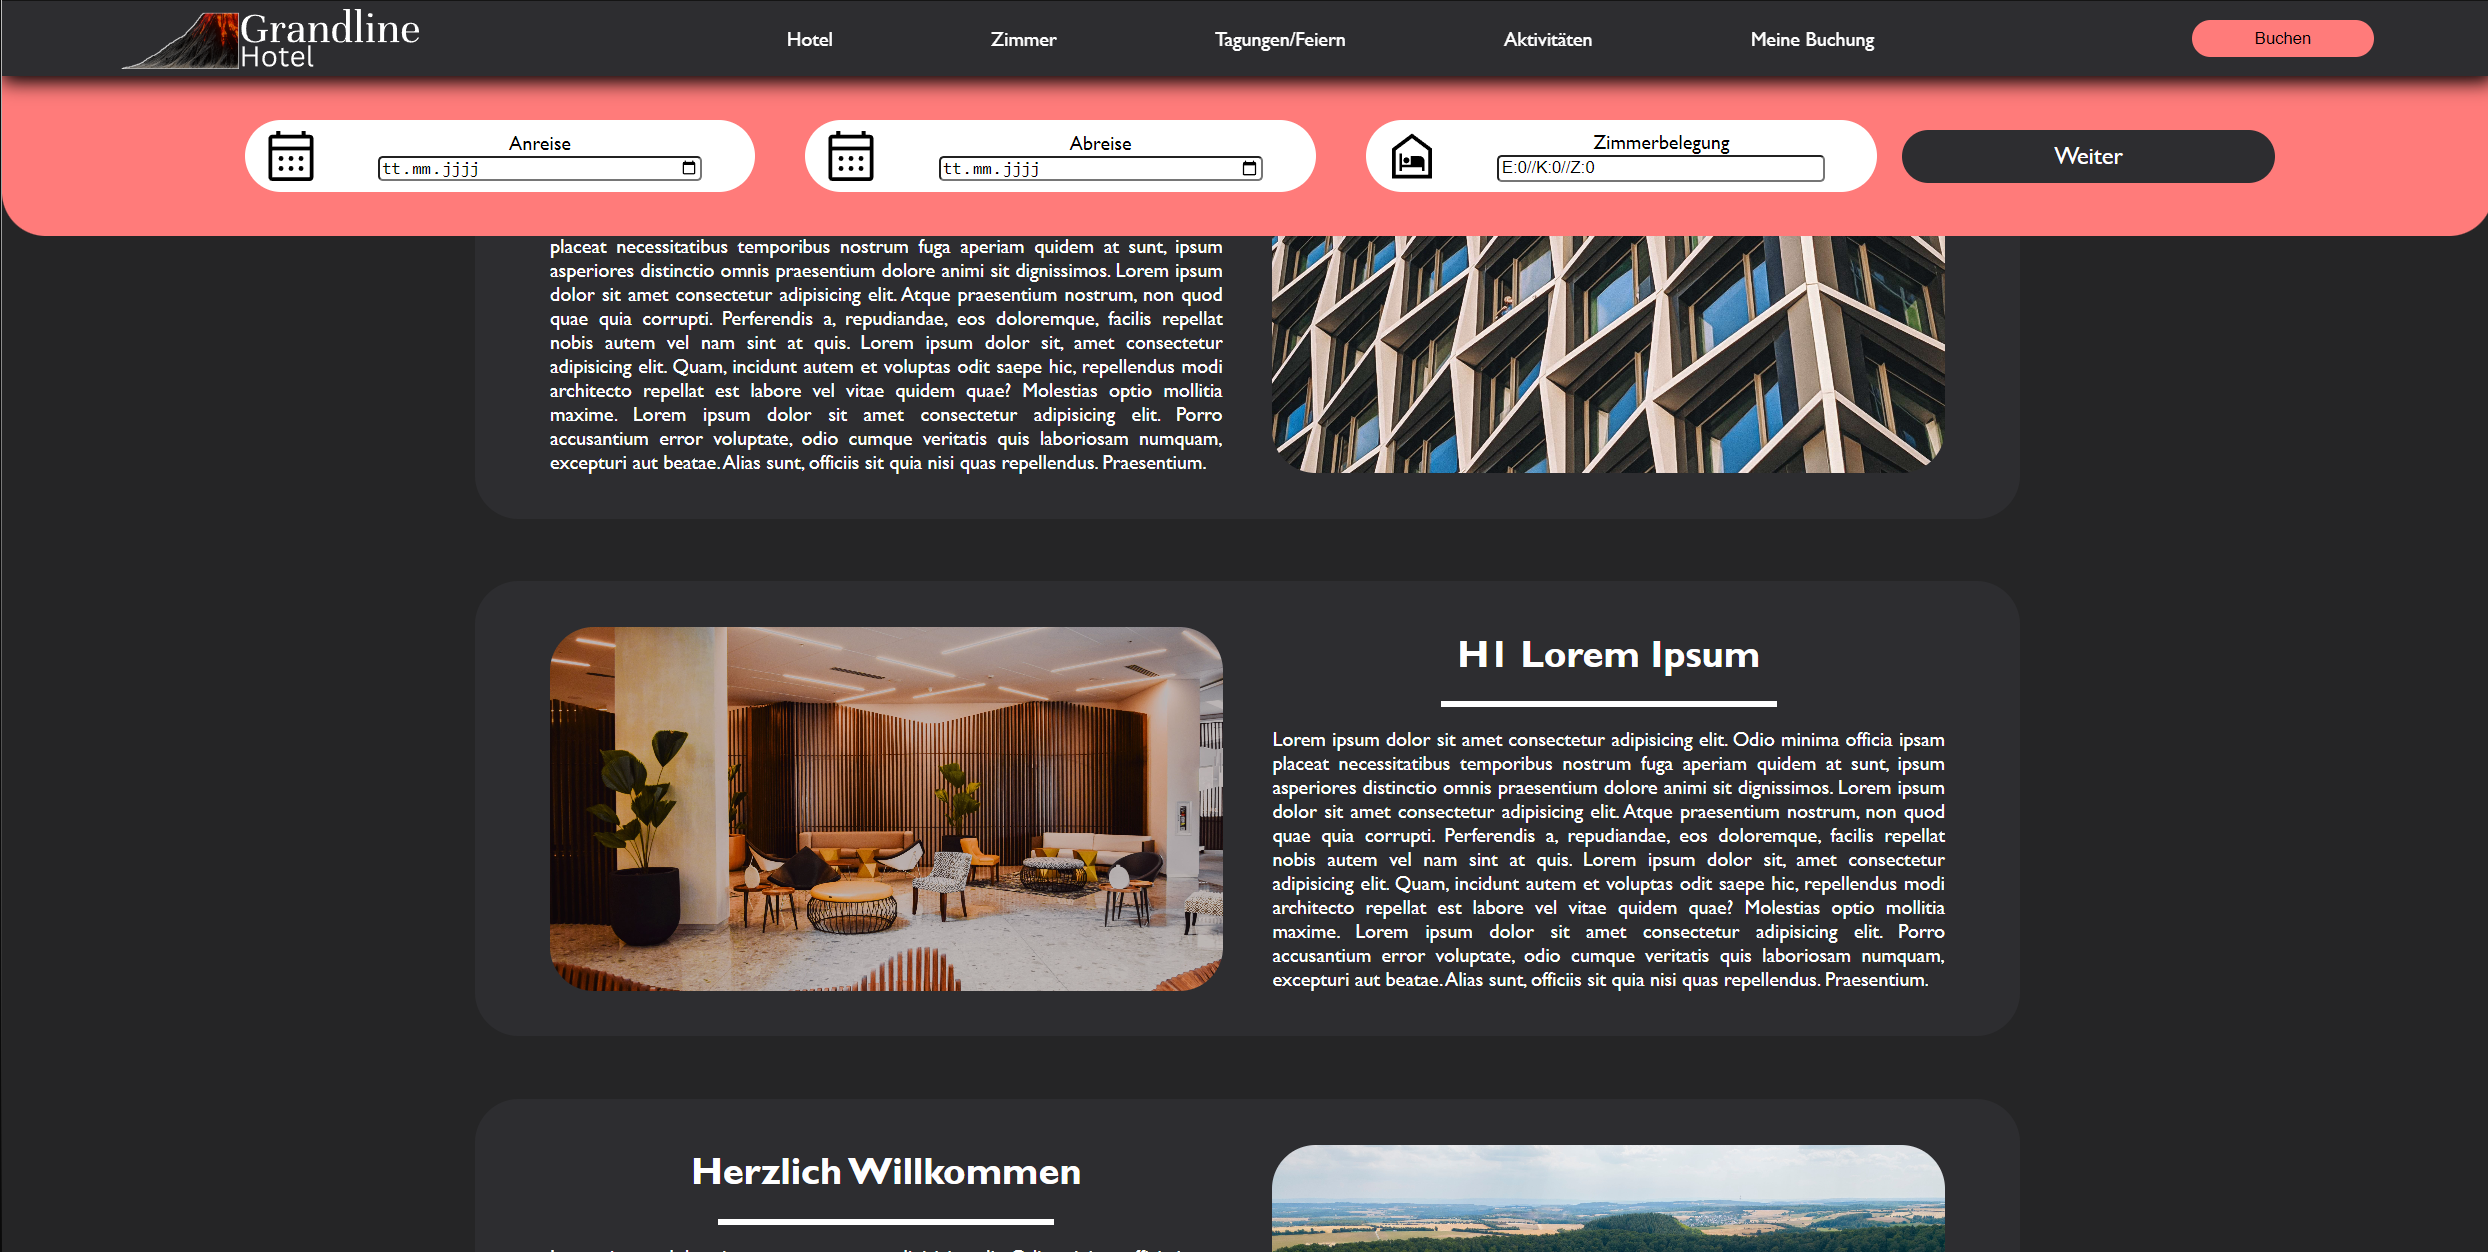
\includegraphics[width=\textwidth]{images/Beispiel/Schritt2.png}
	\caption{Schritt 2}
	\label{step2}
\end{figure}
\newpage In dem 3.Schritt tätigt der Nutzer seine Angaben in das Formular und setzt durch einen Klick auf den \glqq weiter\grqq-Knopf mit der Buchung fort (siehe Abb.\ref{step3}).
\begin{figure}
	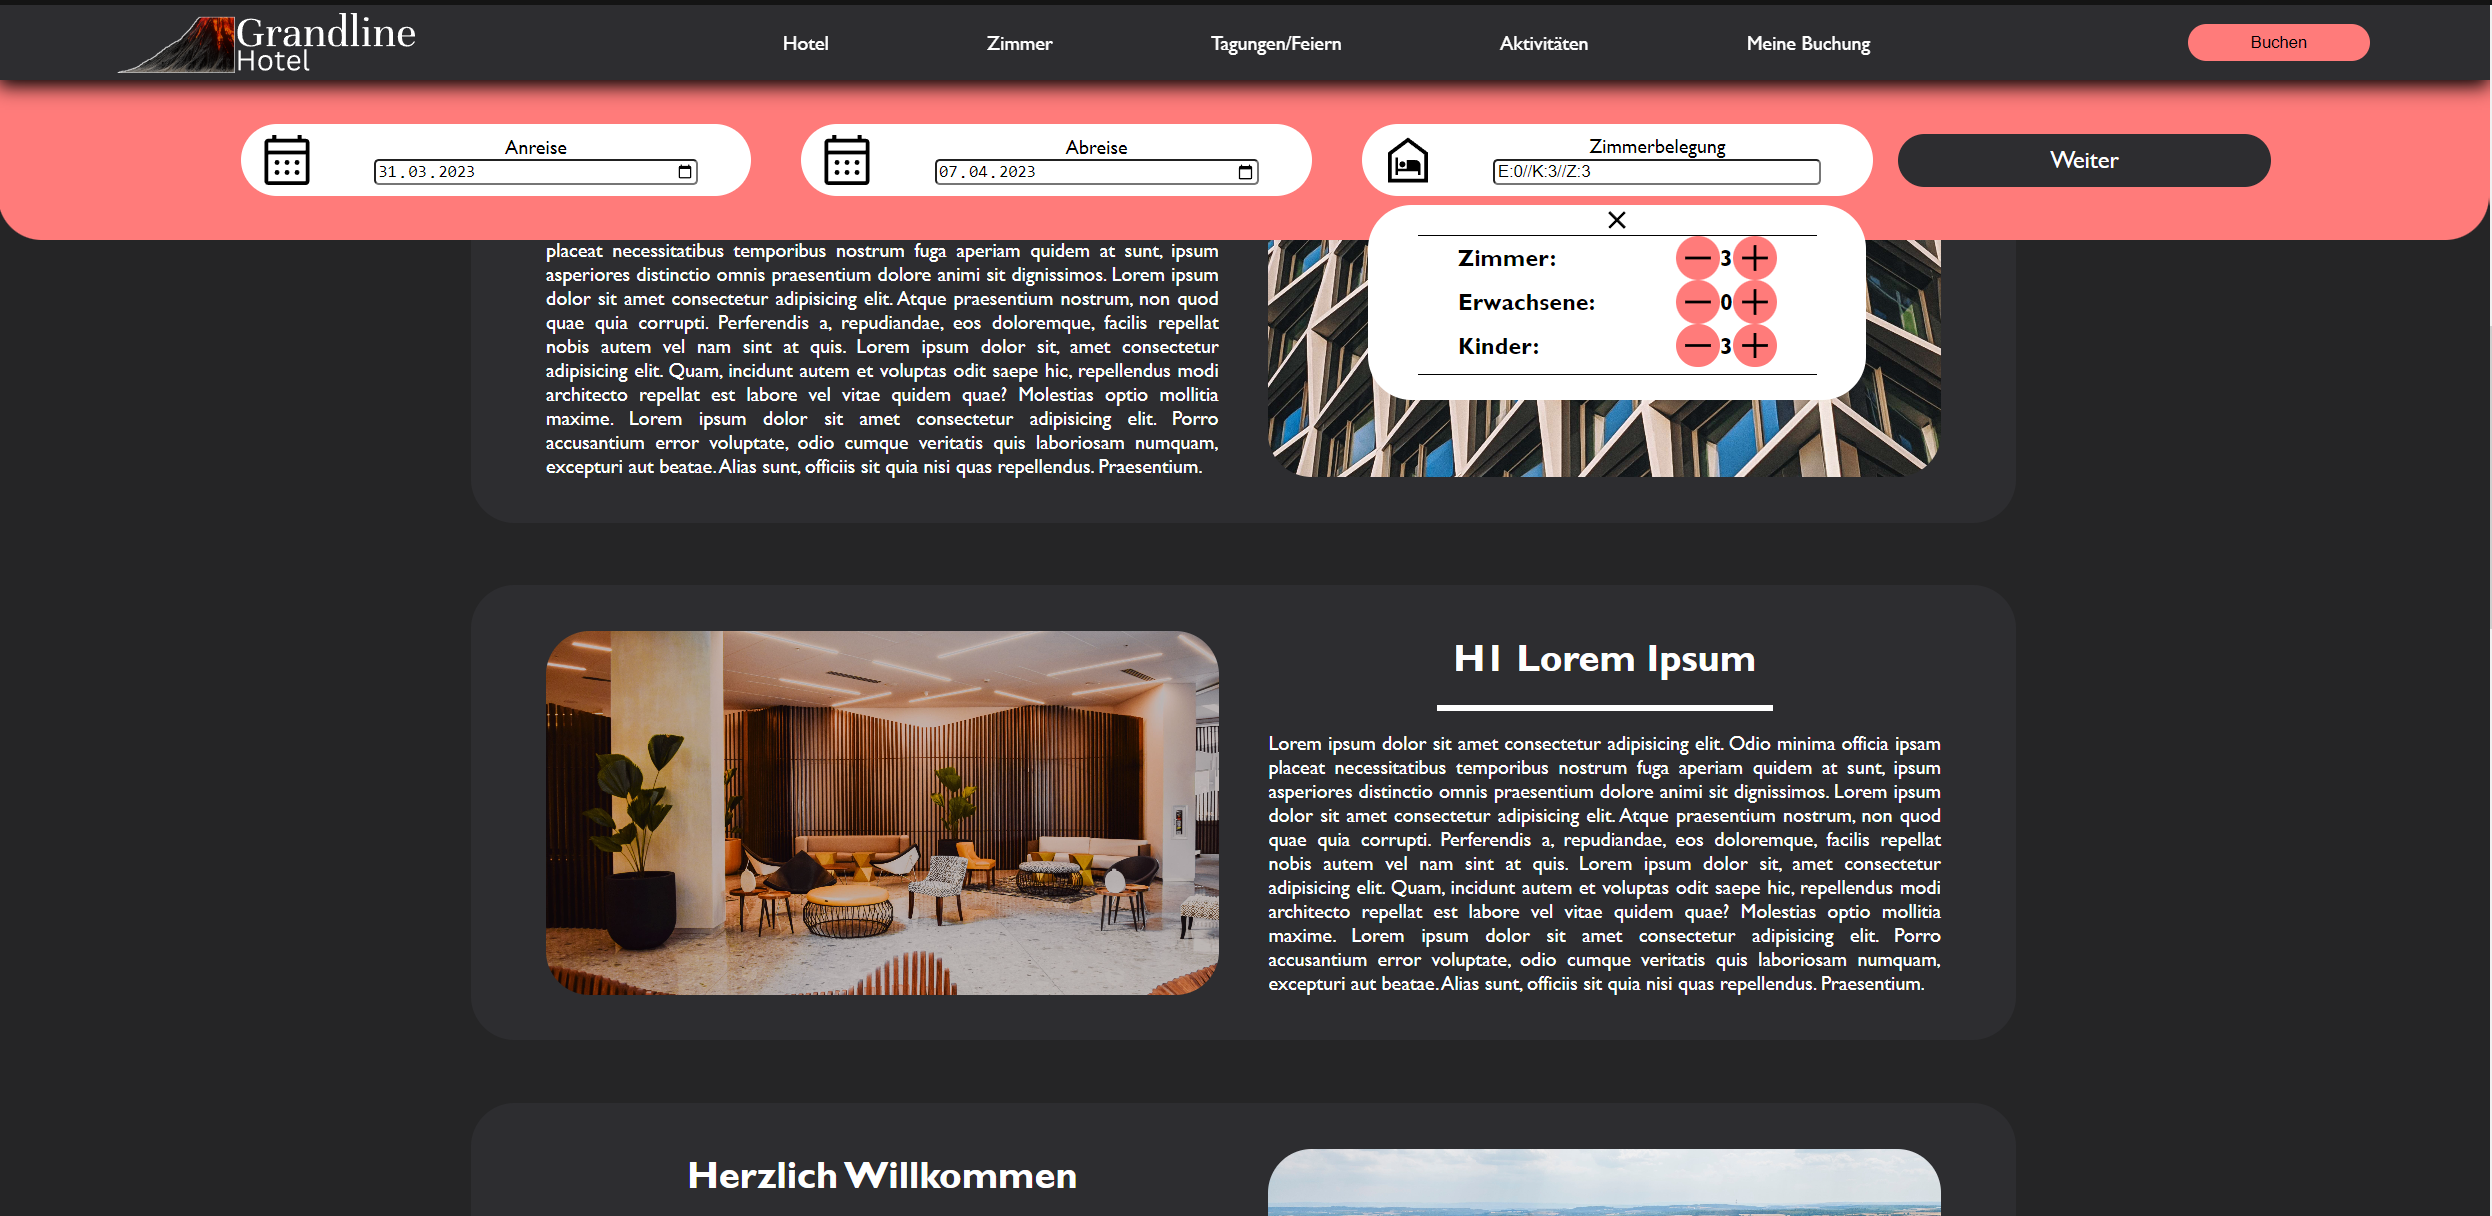
\includegraphics[width=\textwidth]{images/Beispiel/Schritt3.png}
	\caption{Schritt 3}
	\label{step3}
\end{figure}
\newline
Der Nutzer wird nun in den Buchungsdialog weitergeleitet in dem er eine Auswahl der verfügbaren Zimmer dargeboten bekommt (siehe Abb.\ref{step4}).
\begin{figure}
	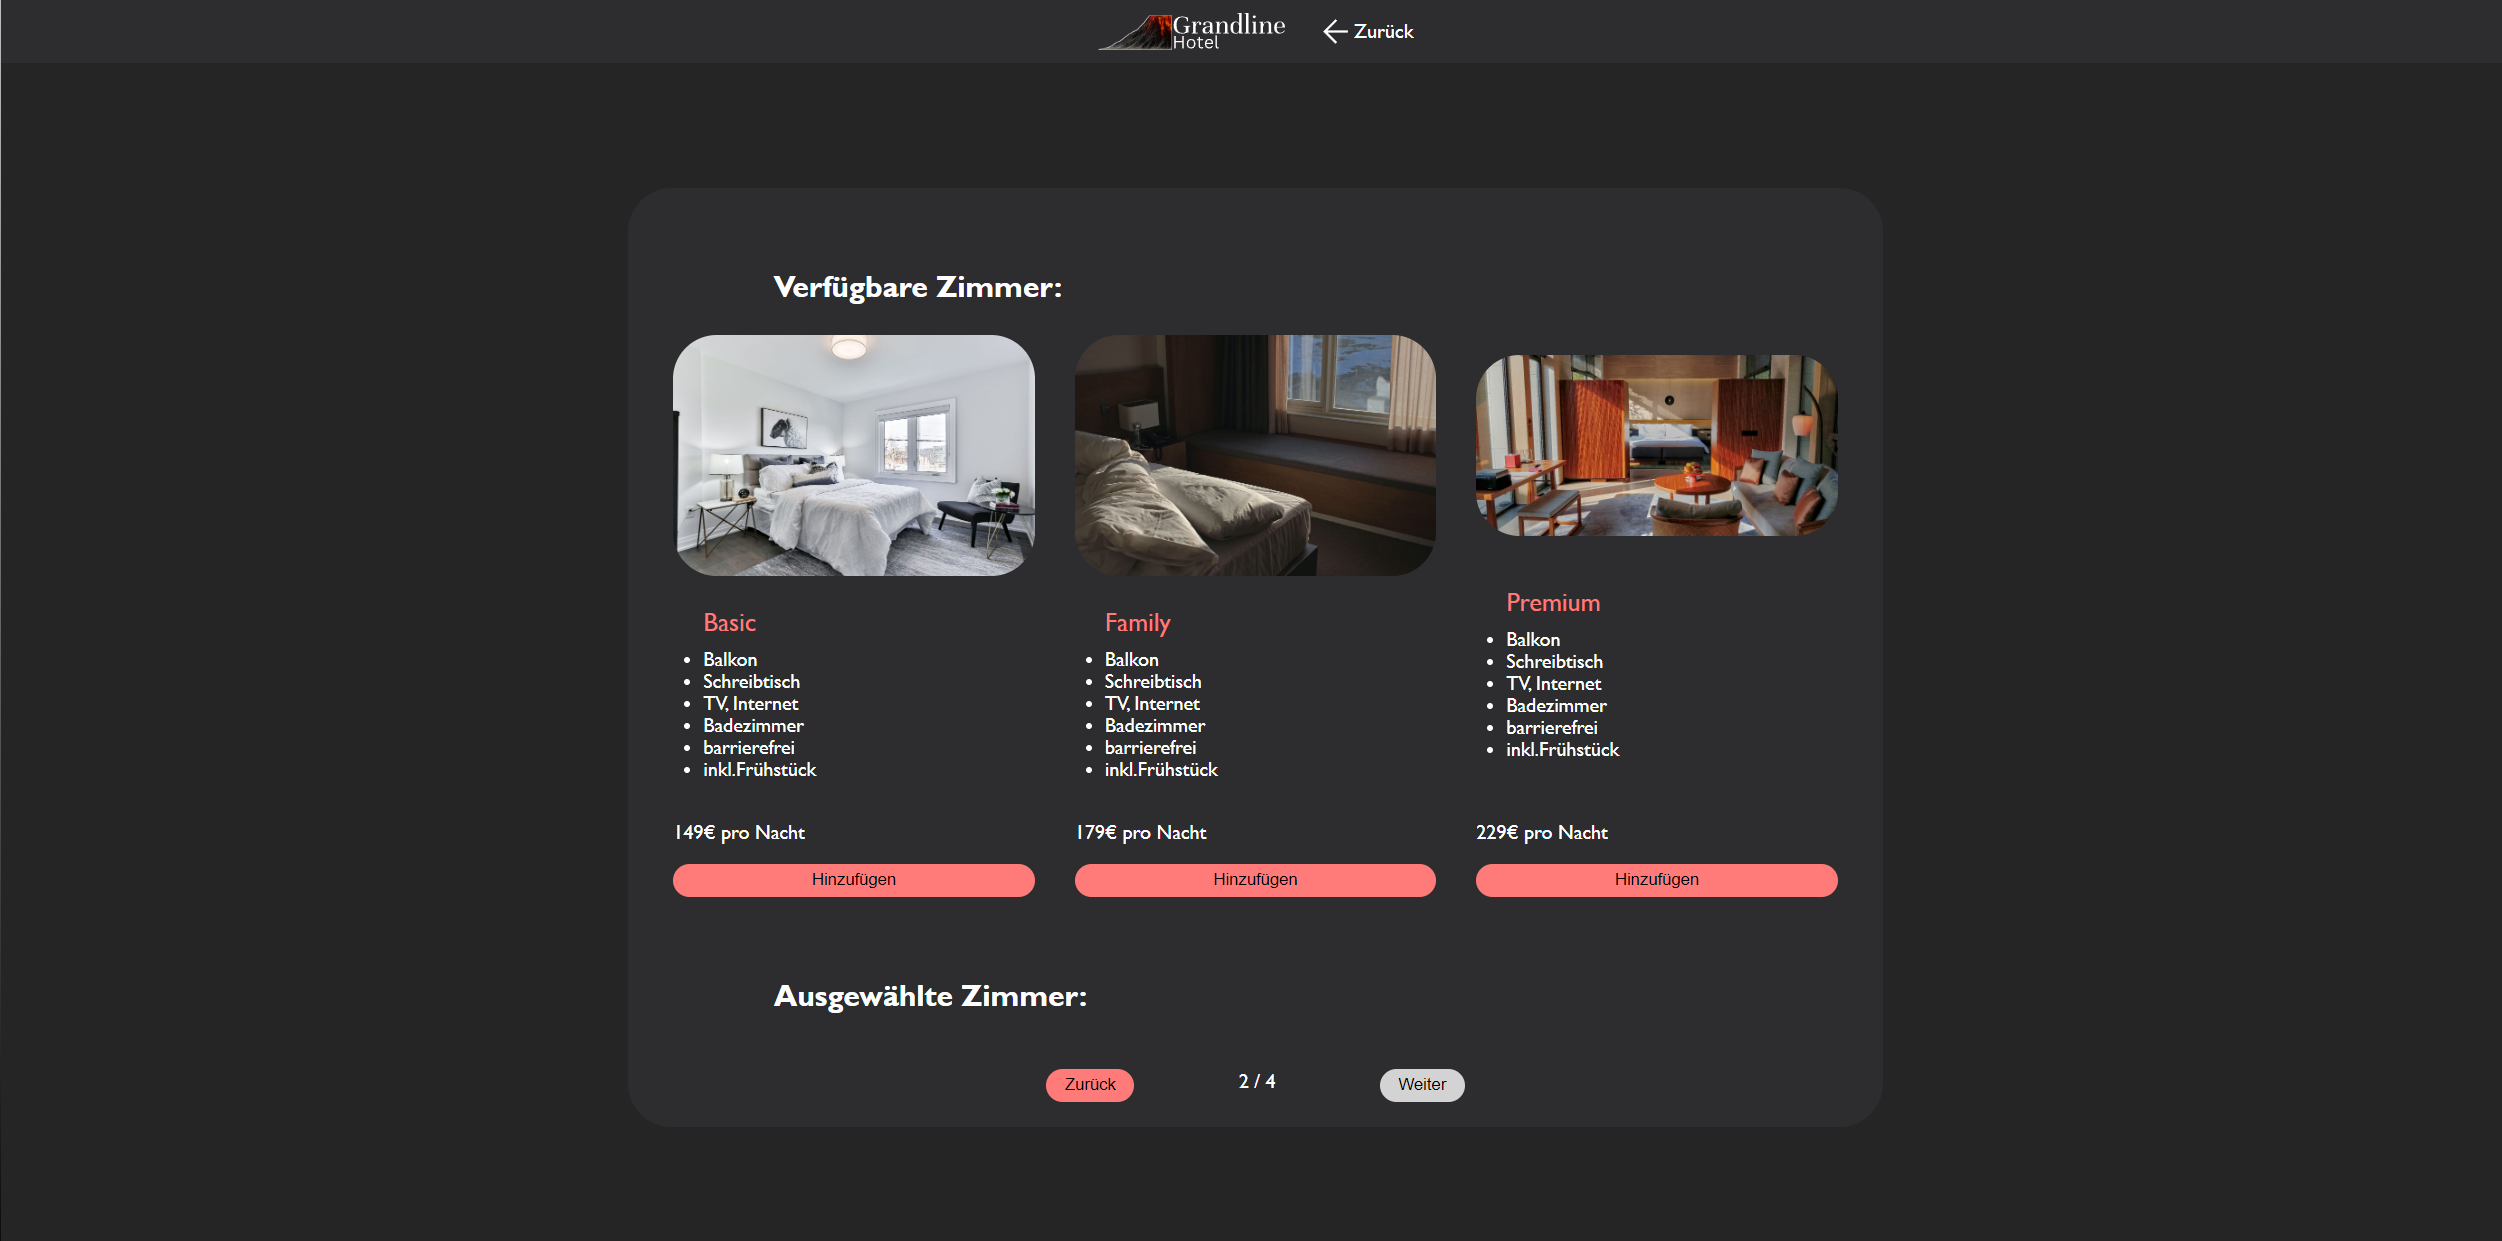
\includegraphics[width=\textwidth]{images/Beispiel/Schritt4.png}
	\caption{Schritt 4}
	\label{step4}
\end{figure}
\newpage
Der Nutzer wählt im 5. Schritt aus den verfügbaren Zimmern die Gewünschten aus und betätigt die \glqq Weiter\grqq-Taste (siehe Abb.\ref{step5}). Die Menge die der Nutzer auswählen muss entspricht der angegebenen Anzahl der Zimmer aus Schritt 3.
\begin{figure}
	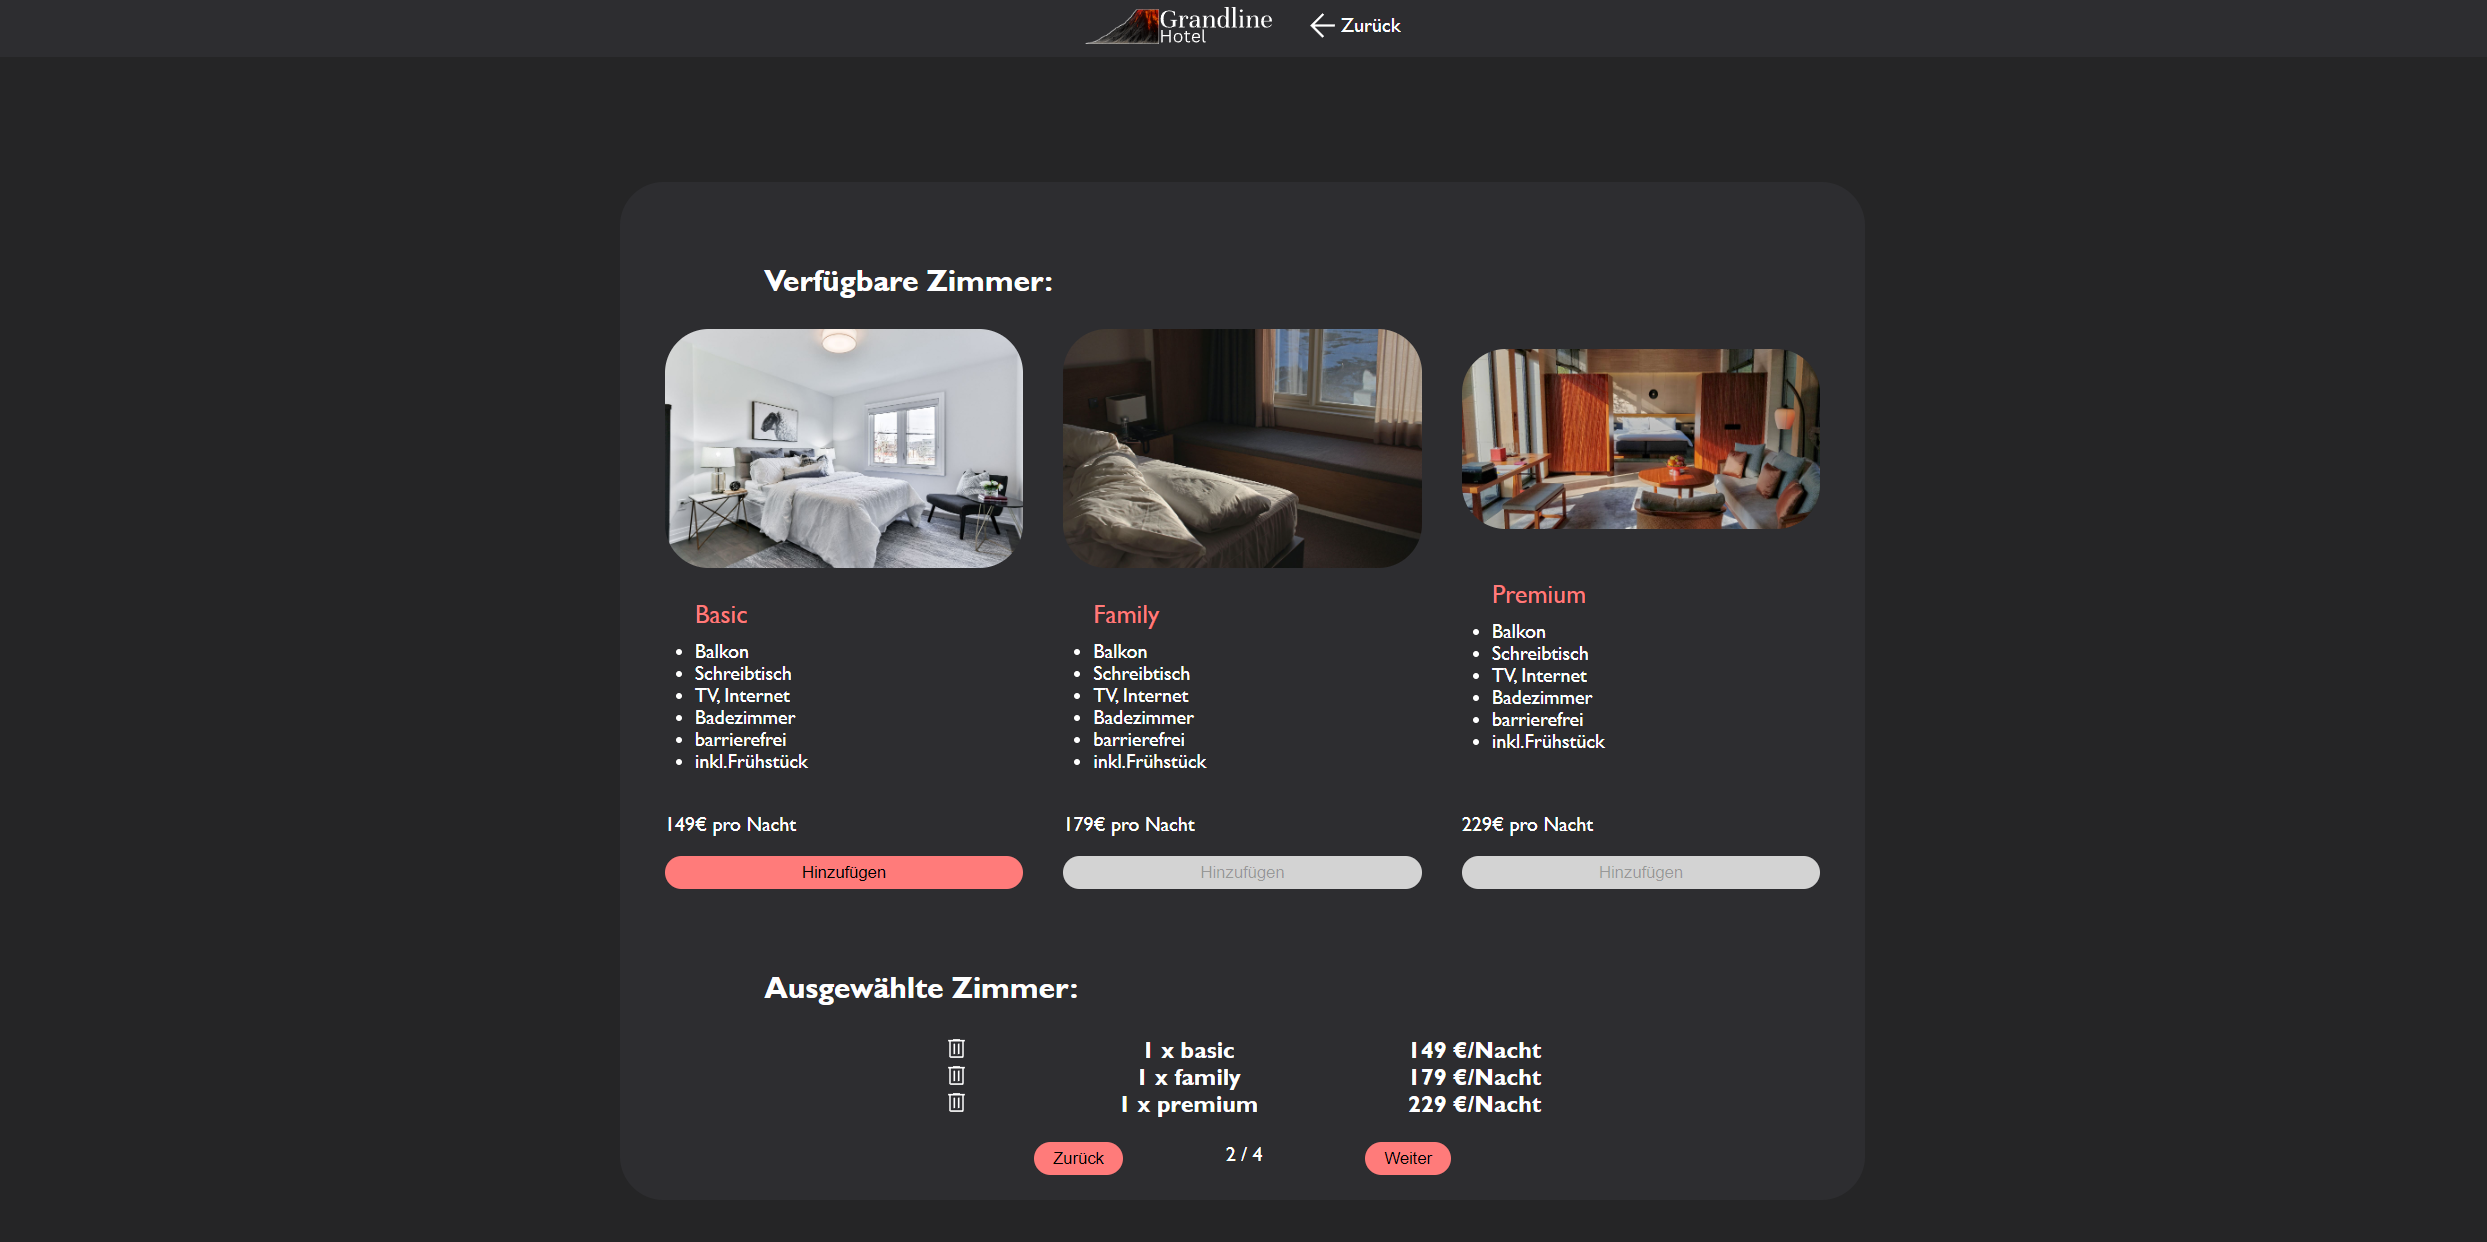
\includegraphics[width=\textwidth]{images/Beispiel/Schritt5.png}
	\caption{Schritt 5}
	\label{step5}
\end{figure}
\newpage
In das nun erschienene Formular trägt der Nutzer seine persönlichen Daten ein und fährt über den \glqq Weiter\grqq-Knopf mit dem Buchungsdialog fort (siehe Abb.\ref{step6}).
\begin{figure}
	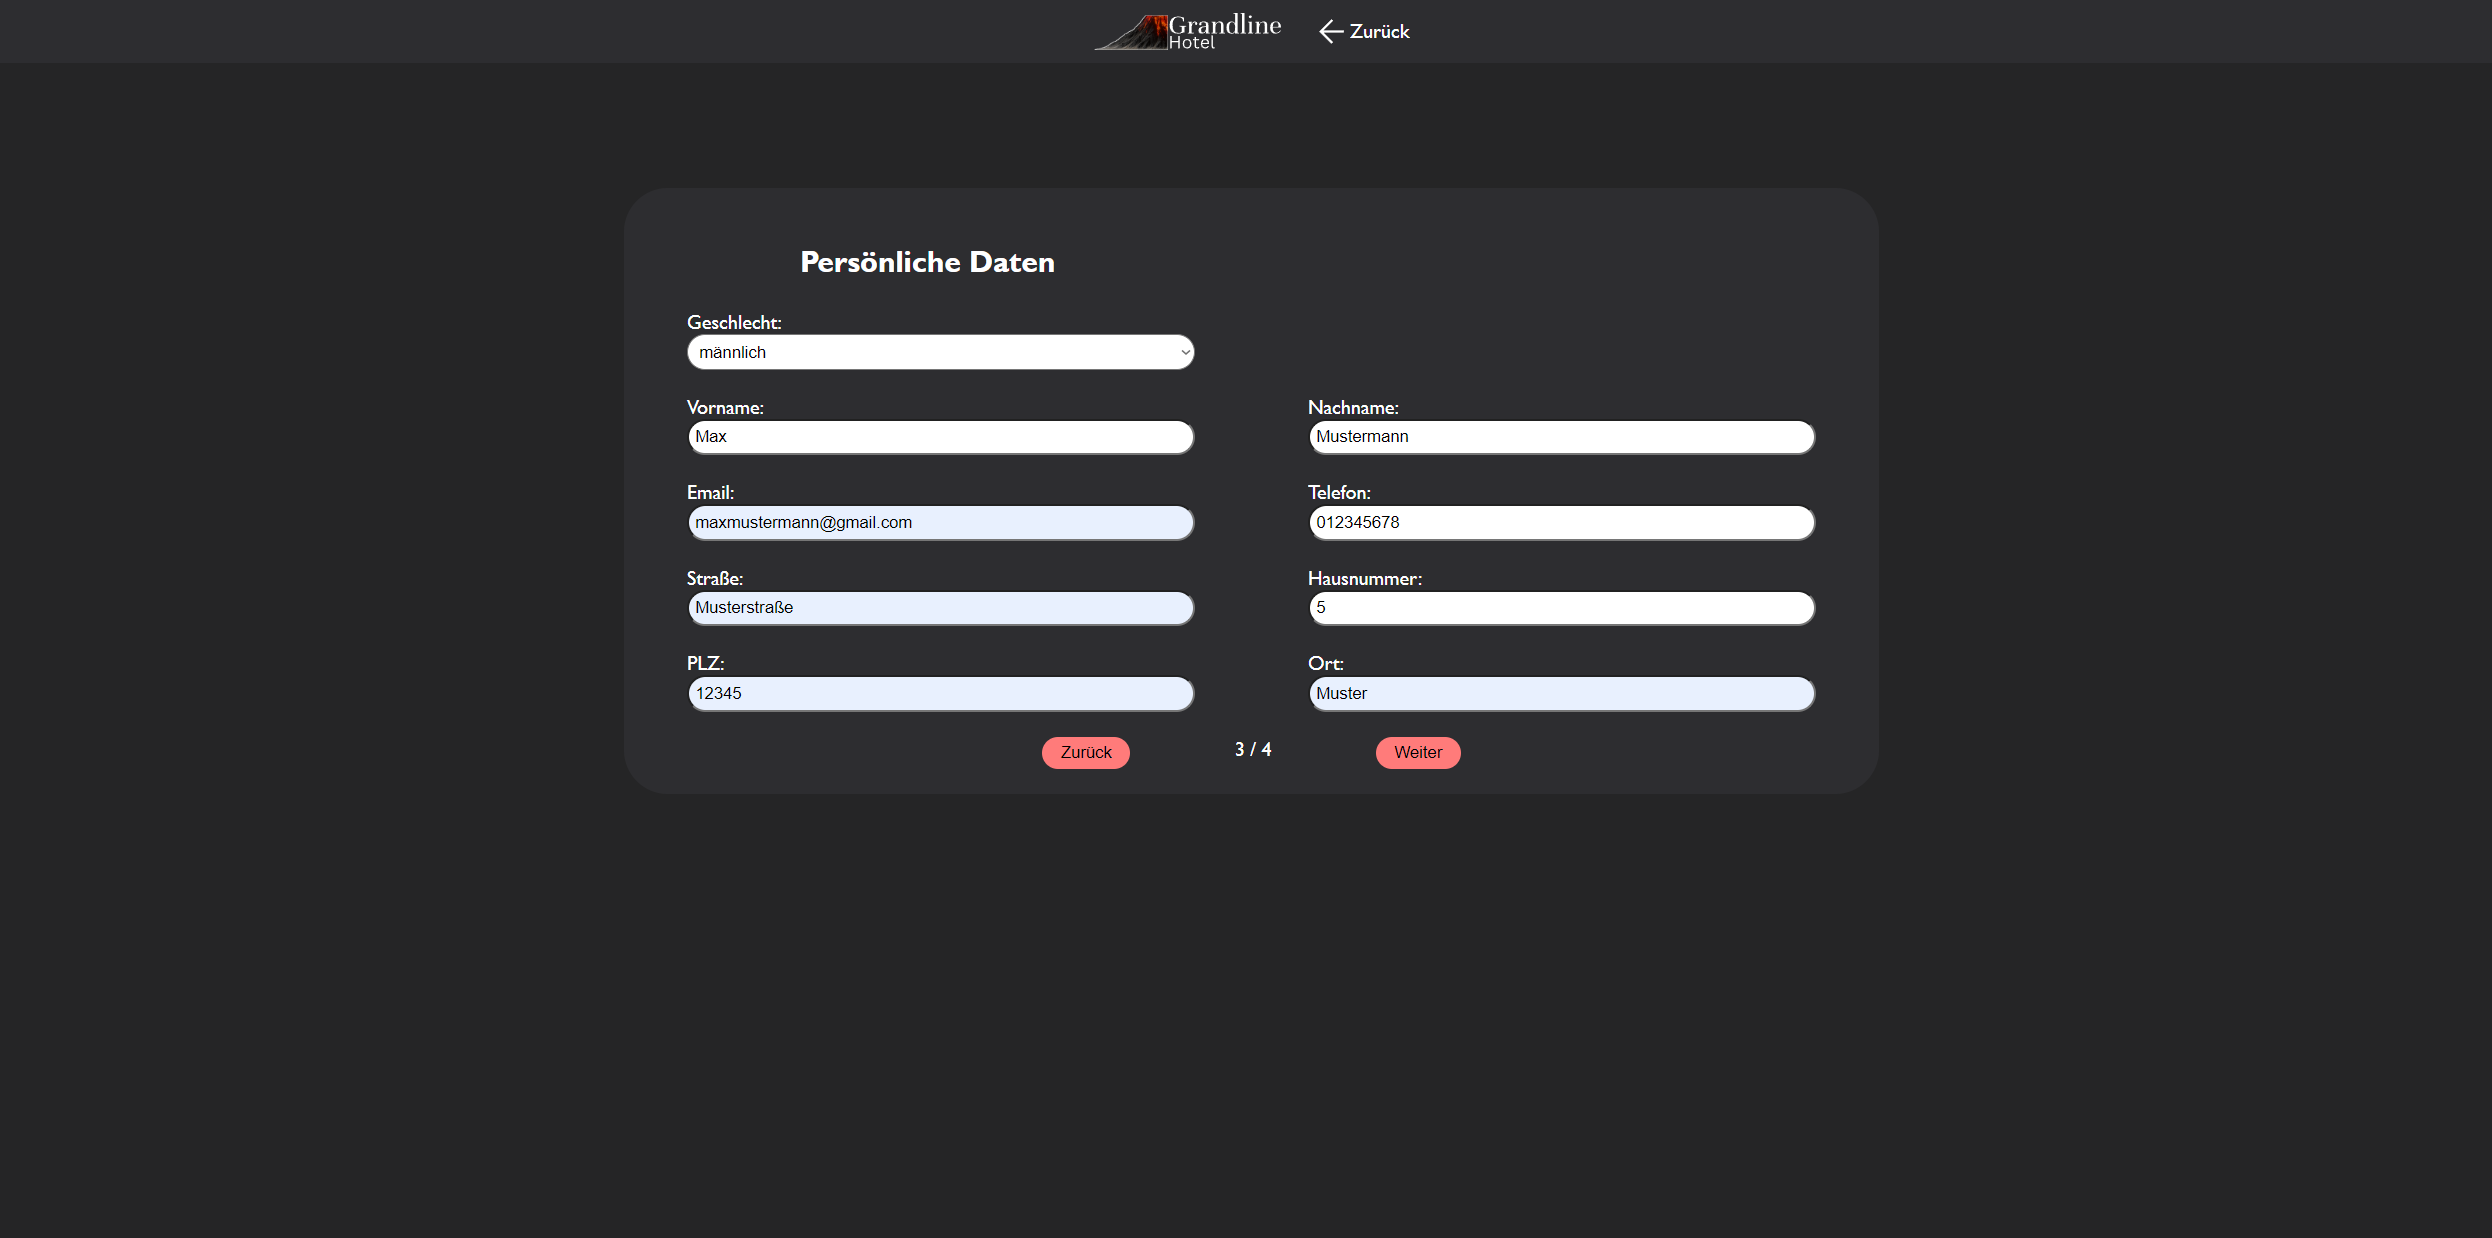
\includegraphics[width=\textwidth]{images/Beispiel/Schritt6.png}
	\caption{Schritt 6}
	\label{step6}
\end{figure}
\newline
Im siebten Schritt wird dem Nutzer eine Übersicht über die zu tätigende Buchung dargeboten und bietet dem Nutzer vor dem Abschluss die Möglichkeit noch Extrawünsche und Informationen über ein Textfeld an das Hotel weiterzugeben (siehe Abb.\ref{step7}). Klickt der Nutzer anschließend auf \glqq Abschließen\grqq, wird der Buchungsprozess abgeschlossen.
\begin{figure}
	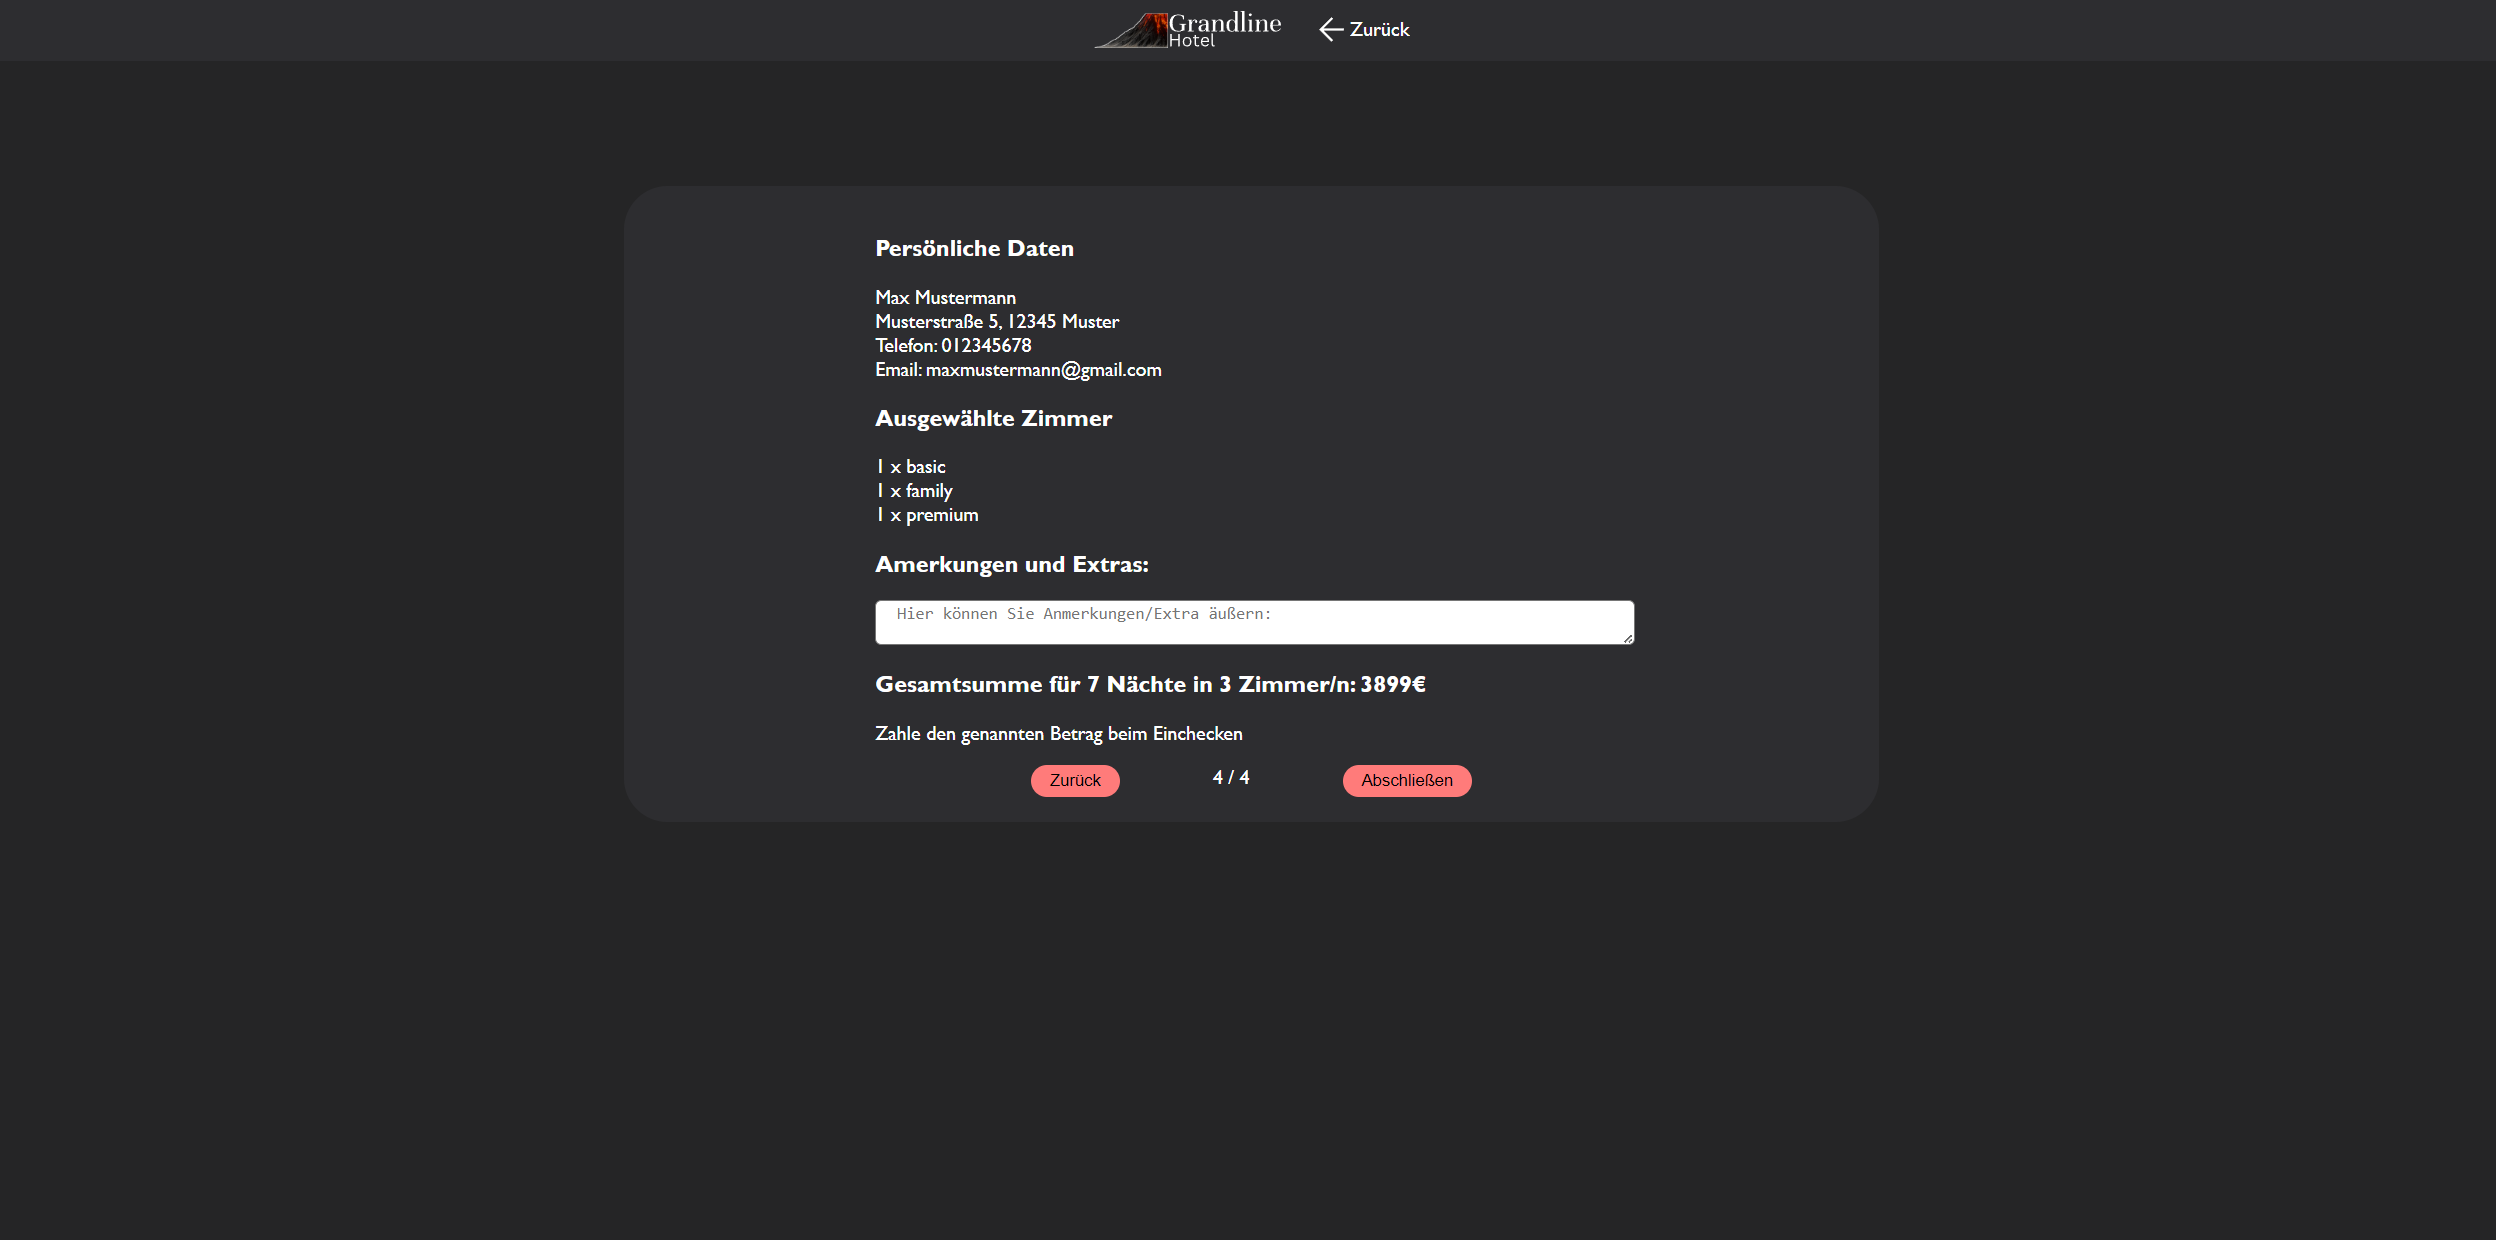
\includegraphics[width=\textwidth]{images/Beispiel/Schritt7.png}
	\caption{Schritt 7}
	\label{step7}
\end{figure}
\newpage
Nach Abschluss der Buchung wird der Nutzer darüber informiert, dass eine E-Mail mit den wichtigsten Informationen an den Nutzer versendet wurde (siehe Abb.\ref{step8}).
\begin{figure}
	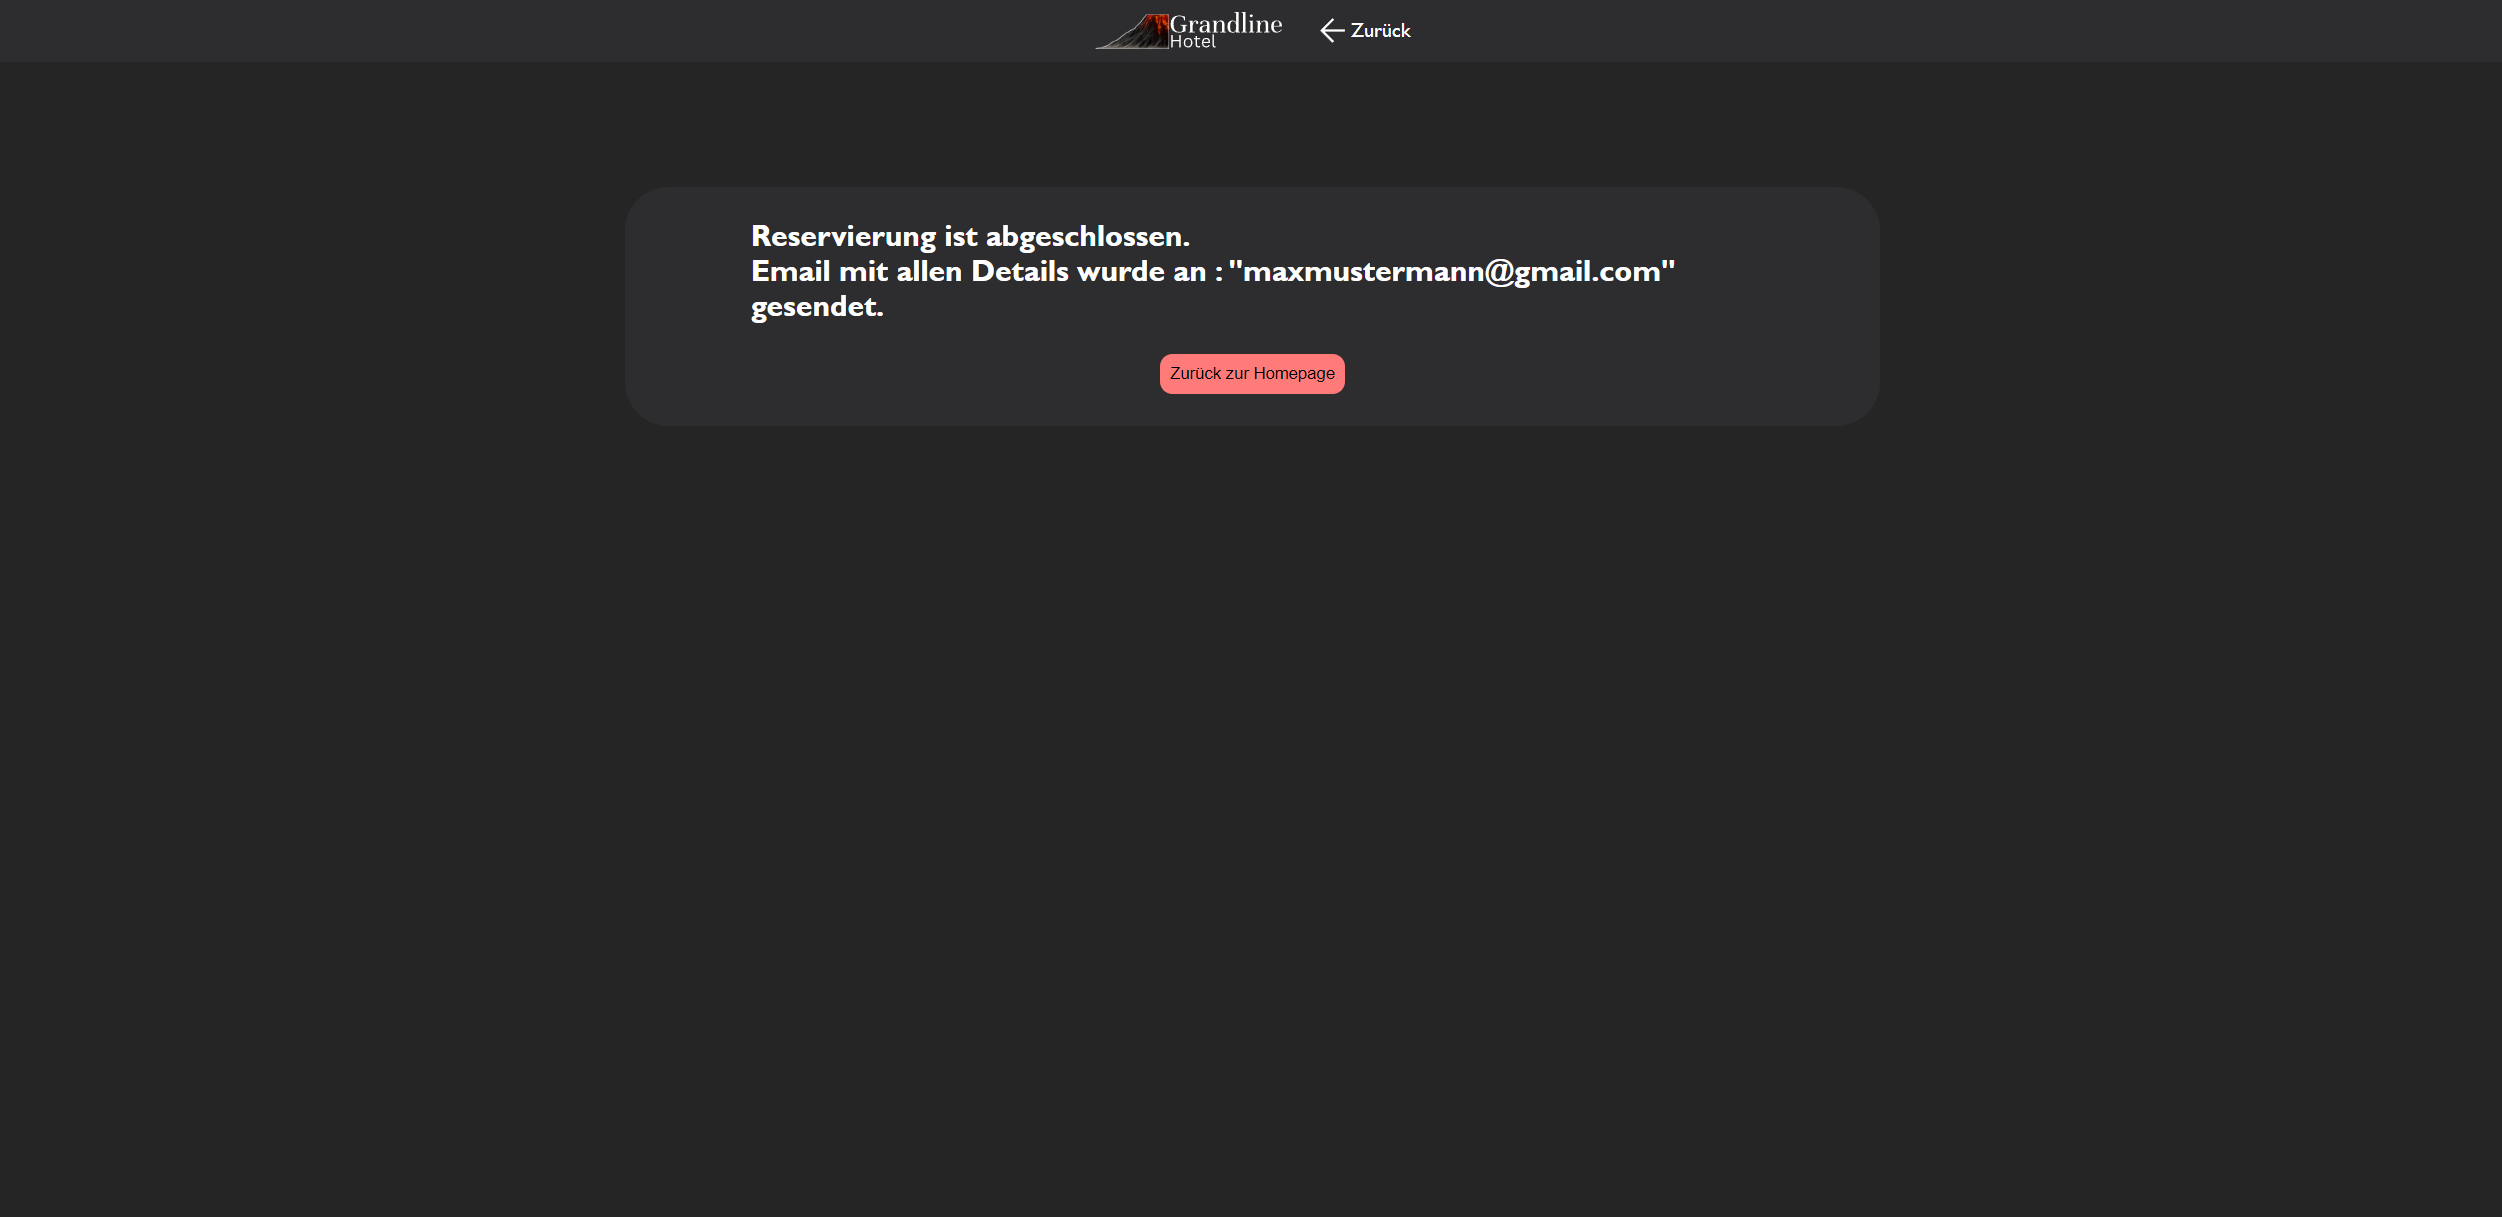
\includegraphics[width=\textwidth]{images/Beispiel/Schritt8.png}
	\caption{Schritt 8}
	\label{step8}
\end{figure}
\chapter{Anwendungsszenarien}
Ein allgemeines Buchungssystem macht nicht nur im Zusammenhang mit Hotels, sondern in vielen weiteren Anwendungen und Branchen Sinn. So kann beispielsweise ein Restaurant ein ähnliches System zur Reservierung von Tischen verwenden. Auch in der Veranstaltungsbranche kann von einem solchen System profitiert werden indem es Nutzern ermöglicht wird Veranstaltungen anzumelden und zu verwalten. Hierzu könne man auch noch eine Funktion zur Anmeldung und Verwaltung von Teilnehmern implementieren. Eine weitere Branche die Gebrauch von solchen Systemen macht ist die der Reisebuchungen. So könnten beispielsweise Flüge, Mietwagen usw. für Kunden gebucht werden. Das System lässt sich also viele Anpassungen für etliche weitere Anwendungen umändern und zeigt so den großen Nutzen.
\chapter{Zusammenfassung und Ausblick}
Das Buchungssystem besteht aus einer clientseitigen Anwendung und einer serverseitigen API. Über die API können Nutzer mittels HTTP-Anfragen Buchungen erstellen, ändern und löschen. Die serverseitige Implementierung erfolgt mit Express und ist dadurch vereinfacht. Zur Sicherung der Buchungsdaten wird eine MongoDB-Datenbank verwendet mit die der Server kommuniziert. Für die Erstellung von Buchungen steht dem Nutzer auf der Client-Seite ein Buchungsdialog zur Verfügung, der mithilfe von den gängigen Front-End-Tools wie HTML, Less und JavaScript umgesetzt wurde. Die Umsetzung des Systems ist ohne großen Aufwand gelungen und erfüllt die Ziele der Arbeit. Insgesamt kann die Implementierung eines Buchungssystems unter Verwendung von Node.js eine robuste und skalierbare Lösung zur Verwaltung von Buchungen bieten. Darauf aufbauend könne man in die Buchung von Zimmern außerdem das Auswählen von Extras hinzufügen.



%------------------ Literaturverzeichnis & Index -------------------------------
\backmatter
\bibliography{literatur}								% Literaturverzeichnis (literatur.bib)
\printindex												% Index (optional)


%------------------ Anhänge ----------------------------------------------------
\begin{appendix}
	\chapter{Selbstständigkeitserklärung}

\begin{description}

\item[$\Box$] Diese Arbeit habe ich selbstständig verfasst und keine anderen als die angegebenen Quellen und Hilfsmittel verwendet.\\

\item[$\Box$] Diese Arbeit wurde als Gruppenarbeit angefertigt. Meinen Anteil habe ich selbstständig verfasst und keine anderen als die angegebenen Quellen und Hilfsmittel verwendet.\\

Namen der Mitverfasser:
\vspace{3cm}

Meine eigene Leistung ist:
\vspace{3cm}

\end{description}

\vspace{3cm}

\begin{minipage}[t]{3cm}
	\rule{3cm}{0.5pt}
	Datum
\end{minipage}
\hfill
\begin{minipage}[t]{9cm}
	\rule{9cm}{0.5pt}
	Unterschrift der Kandidatin/des Kandidaten
\end{minipage}
	% Selbstständigkeitserklärung
\end{appendix}


\end{document}
